\documentclass[aspectratio=169]{beamer}
\usepackage{minted}
\usepackage{listings}
\usepackage{tikz}
\usetikzlibrary{shapes,arrows}
\usetheme{metropolis}
\title{Programming Languages and Trust}
\subtitle{The what, why, and how (and the hacks)}
\date{\today}
\author{Veit Heller}
\institute{Datengarten | CCCB}
\tikzstyle{block} = [draw, fill=blue!20, rectangle,
    minimum height=3em, minimum width=6em]
\tikzstyle{input} = [coordinate]
\tikzstyle{output} = [coordinate]
\begin{document}
  \maketitle
  \begin{frame}{\texttt{whoami}}
    \begin{itemize}
      \item I work at a consultancy.
      \item I hack on languages in my free time.
      \item zepto, Carp, cspfuck\ldots
      \item I’m secretly a turtle.
    \end{itemize}
  \end{frame}
  \section{Compilers}
  \begin{frame}{How do programming languages work?}
    \begin{itemize}
      \item We usually start with a messy dichotomy and juxtapose compilers and interpreters.
      \begin{itemize}
        \item Compilers transform source code into some form of executable code.
        \item Interpreters take in source code and evaluate it directly.
      \end{itemize}
    \end{itemize}
  \end{frame}
  \begin{frame}{How do programming languages really work?}
    \begin{itemize}
      \item Most “real” implementations transform their source code first in some way.
      \item This representation has many names: Abstract Syntax Tree (AST), Intermediate Representation (IR), Byte Code, Bit Code, et al.
      \item And what about transpilers? Oh my.
    \end{itemize}
  \end{frame}
  \begin{frame}{How do programming languages really work?}
    \begin{itemize}
      \item We have some sort of pipeline:
      \begin{itemize}
        \item Takes in source code,
        \item Transforms, and
        \item Spits out another representation or evaluates it directly.
      \end{itemize}
    \end{itemize}
  \end{frame}
  \begin{frame}{A pipeline?}
    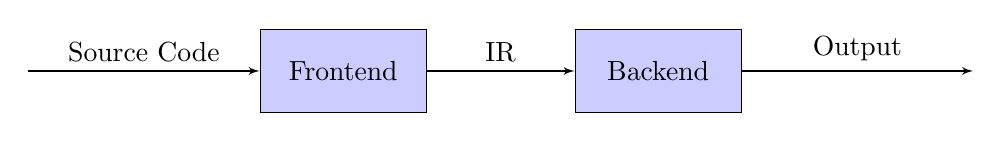
\begin{tikzpicture}[auto, node distance=4cm,>=latex']
        \node [input, name=input] {};
        \node [block, right of=input] (frontend) {Frontend};
        \node [block, right of=frontend] (backend) {Backend};
        \node [output, right of=backend] (output) {};

        \draw [draw,->] (input) -- node {Source Code} (frontend);
        \draw [->] (frontend) -- node {IR} (backend);
        \draw [->] (backend) -- node [name=Output] {Output}(output);
    \end{tikzpicture}
  \end{frame}
  \begin{frame}[fragile]
    \frametitle{A pipeline?}
    \begin{listing}[H]
      \caption{A silly Brainfuck VM}
      \begin{minted}[fontsize=\scriptsize]{c}
void eval(char* str) {
  int tape[30000];
  int head = 0;
  for (int i = 0; i<30000; i++) tape[i] = 0;
  while(*str) {
    switch(*str) {
      case '+': tape[head]++; break;
      case '-': tape[head]--; break;
      case '>': head++; break;
      case '<': head--; break;
      case '.': printf("%c", tape[head]); break;
      case ',': scanf("%c", (char*)&tape[head]); break;
      case '[': if(!tape[head]) str = search_end_loop(str); break;
      case ']': if(tape[head]) str = search_begin_loop(str); break;
    }
    ++str;
  }
}
      \end{minted}
    \end{listing}
  \end{frame}
  \begin{frame}[fragile]
    \frametitle{A pipeline?}
    \begin{figure}
      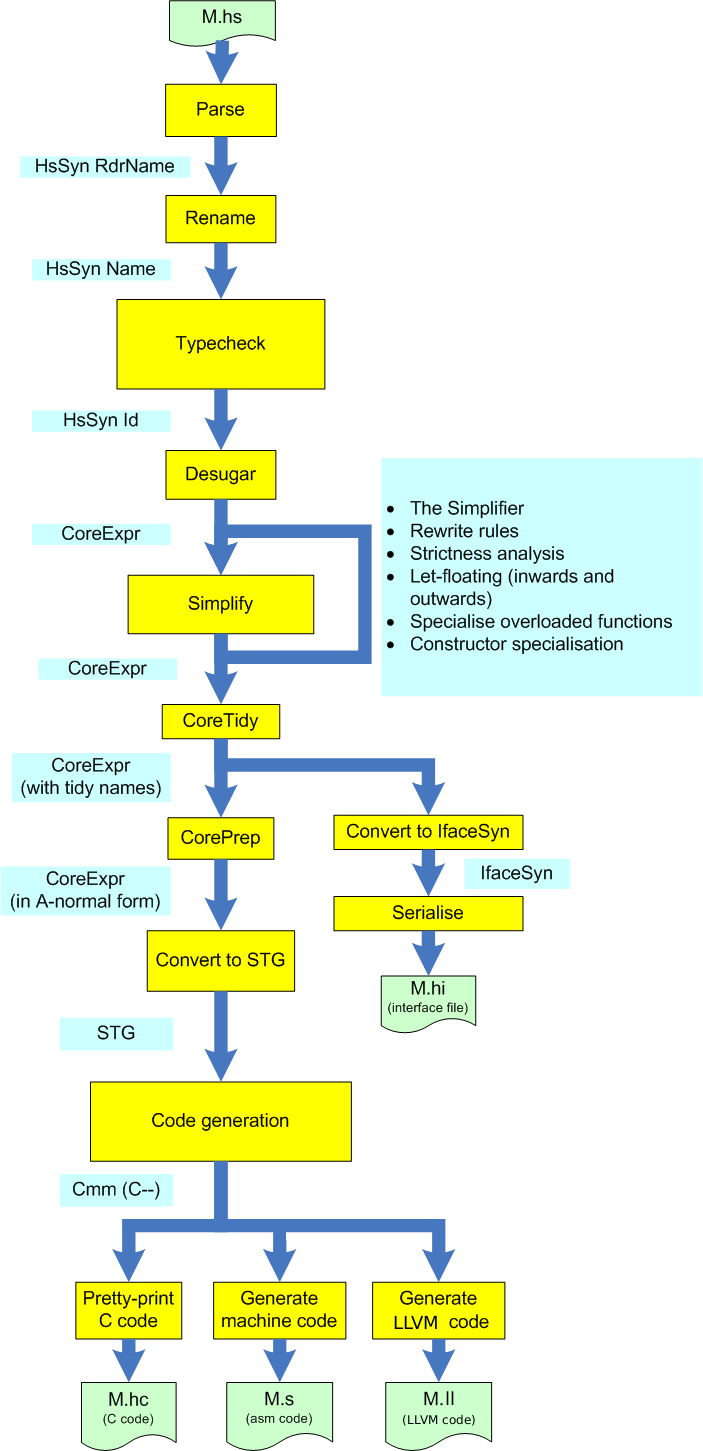
\includegraphics[height=5.4cm]{ghc_pipeline.png}
      \caption{The GHC pipeline.}
    \end{figure}
    \scriptsize This picture was sourced from https://ghc.haskell.org/trac/ghc/wiki/Commentary/Compiler/HscMain.
  \end{frame}
  \begin{frame}{Why pipelines?}
    \begin{itemize}
      \item Huge pipelines like this might seem overkill for simple languages.
      \item These days, they buy us modularity, clarity, and a low barrier of entry.
      \item Independent passes are great! I can finally do proper testing!
      \item The extreme end of this spectrum is nanopass compilers (cool stuff!).
    \end{itemize}
  \end{frame}
  \begin{frame}{Passes Frontend—Tokenizer/Lexer/Parser}
    \begin{itemize}
      \item Most language implementations have a parser.
      \item Tokenizer/Lexer splits stream up into tokens (Lex/Flex/ANTLR...).
      \item Parser generates IR/AST from source or tokens.
    \end{itemize}
  \end{frame}
  \begin{frame}{Passes Frontend—Tokenizer/Lexer/Parser}
    \begin{itemize}
      \item Parsers are generally more interesting.
      \item You can generate them (YACC/Bison/ANTLR...)—but that’s boring.
      \item You can alse write them completely manually (recursive descent is
            popular) or use a framework.
      \item Personal favorites: recursive descent, GLL (Generalized
            Left-to-Right, Leftmost derivation), OMeta, Parsec.
      \item Rule of Thumb: Don’t overengineer it early on. It’s easy to replace.
    \end{itemize}
  \end{frame}
  \begin{frame}{Passes Frontend—Typechecking}
    \begin{itemize}
      \item You can have fun with types!
      \item A simple, but powerful model is Hindley-Milner, with sum and product
            types (think Haskell or OCaml).
      \item It buys you a “simple” type inference algorithm for functions.
      \item You can go wild! Dependent types, Liquid Types, and a whole bunch of
            things I don’t understand!
      \item You don’t need a pass for that, but even in dynamic languages
            sometimes this makes sense because specialization leads to better
            generated code.
    \end{itemize}
  \end{frame}
  \begin{frame}{Passes Backend—Optimizations}
    \begin{itemize}
      \item Heavily language-dependent!
      \item[$\Rightarrow$] Example: Haskell is heavily optimized in a way that
                           doesn’t make sense elsewhere—because it is lazy,
                           reordering is extremely important. And don’t forget
                           currying!
      \item It’s not always higher level to lower level; more on that later.
      \item It’s not black magic, although it often feels like it is.
      \item If you use LLVM you already have dozens of passes available to you.
    \end{itemize}
  \end{frame}
  \begin{frame}{Passes Backend—Optimizations}
    What does \texttt{[-]} mean in Brainfuck?
  \end{frame}
  \begin{frame}{Passes Backend—Optimizations}
    It means “set the current value under the tape to zero”.

    \begin{itemize}
      \item[$\Rightarrow$] We can remove the loop entirely!
    \end{itemize}
  \end{frame}
  \section{Demo I—enter cspfuck}
  \section{Trust}
  \begin{frame}{Trusting Trust}
    \begin{itemize}
      \item In 1984, Ken Thompson was rightfully awarded the Turing Award.
      \item He wrote a three-page paper on a scary idea: malicious compilers.
    \end{itemize}
  \end{frame}
  \begin{frame}{The idea}
    \begin{itemize}
      \item Have you heard about Quines? They are self-replicating programs.
      \item Have you heard about bootstrapping compilers? They are compilers
            that can compile themselves.
      \item What if we compile a “buggy” version of our compiler and ship it?
    \end{itemize}
  \end{frame}
  \begin{frame}{The idea}
    If you cannot trust your compiler, all of the programs you compile are
    possibly malicious. It doesn’t even need to compromise existing
    functionality.
  \end{frame}
  \begin{frame}{The idea}
    “The actual bug I planted in the compiler would match code in the UNIX
     "login" command.  The replacement code would miscompile the login
     command so that it would accept either the intended encrypted password
     or a particular known password. Thus if this code were installed in
     binary and the binary were used to compile the login command, I could
     log into that system as any user.”

     \indent — Ken Thompson, Trusting Trust, page 3
  \end{frame}
  \begin{frame}{The idea}
    “Such blatant code would not go undetected for long. Even the most casual
     perusal of the source of the C compiler would raise suspicions.” 

     \indent — Ken Thompson, Trusting Trust, page 3
  \end{frame}
  \begin{frame}{The idea}
    “This [second approach] simply adds a second Trojan horse to the one that
     already exists. The second pattern is aimed at the C compiler. [\ldots] First
     we compile the modified source with the normal C compiler to produce a
     bugged binary. We install this binary as the official C. We can now remove
     the bugs from the source of the compiler and the new binary will reinsert
     the bugs whenever it is compiled. Of course, the login command will remain
     bugged with no trace in source anywhere.”

     \indent — Ken Thompson, Trusting Trust, page 3
  \end{frame}
  \begin{frame}{Takeaways}
    \begin{itemize}
      \item It has historically mostly been regarded as a scary practical joke
            by compiler engineers.
      \item As compilers get more complex (and more modular), a malicious
            “optimization” pass can ever more easily be inserted into the
            compiler.
      \item If someone pointed at an obscure piece of assembly and told you
            that “this simple optimization buys us a 10\% speed gain on
            auto-vectorized code in ARM”, would you just believe them?
    \end{itemize}
  \end{frame}
  \section{Demo II—enter Michael Arntzenius}
  \begin{frame}{References I}
    \begin{itemize}
      \item These slides: \texttt{https://github.com/hellerve/talks}
      \item A talk on Nanopass Compilers by Andrew Keep: \texttt{https://www.youtube.com/watch?v=Os7FE3J-U5Q}
      \item Ken Thompson, Trusting Trust: \texttt{https://www.win.tue.nl/~aeb/linux/hh/thompson/trust.html}
      \item Michael Arntzenius’ reflections on Trusting Trust: \texttt{https://github.com/rntz/rotten}
      \item A blog post on how I sped up cspfuck: \texttt{https://blog.veitheller.de/Speeding\_up\_an\_Interpreter.html}
      \item My favorite talks on compilers and interpreters: \texttt{https://github.com/hellerve/programming-talks\#compilersinterpreters}
      \item Some of my favorite (and loathed) papers: \texttt{https://github.com/hellerve/ptolemy/blob/master/done.md}
      \item A list of LLVM passes: \texttt{http://llvm.org/docs/Passes.html}
    \end{itemize}
  \end{frame}
  \begin{frame}[fragile]
    \frametitle{References II}
    \begin{itemize}
      \item Elizabeth Scott and Adrian Johnstone, GLL Parsing: \texttt{http://dotat.at/tmp/gll.pdf}
      \item Daan Leijen and Erik Meijer, Parsec: Direct Style Monadic Parser Combinators for the Real World: \texttt{https://www.microsoft.com/en-us/research/publication/parsec-direct-style-monadic-parser-combinators-for-the-real-world/}
      \item Ana Bove and Peter Dybjer, Dependent Types at Work: \texttt{http://www.cse.chalmers.se/\%7Epeterd/papers/DependentTypesAtWork.pdf}
      \item Alessandro Warth, Experimenting with Programming Languages (The original thesis on OMeta): \texttt{www.vpri.org/pdf/tr2008003\_experimenting.pdf}
      \item Patrick Rondon et al, Liquid Types: \texttt{http://goto.ucsd.edu/\textasciitilde rjhala/liquid/liquid\_types.pdf}
    \end{itemize}
  \end{frame}
  \begin{frame}{\texttt{exit}}
    \Huge Thank you!
    \linebreak
    \linebreak
    \linebreak
    \small Questions?
    \linebreak
    \linebreak
    \tiny Slides at \texttt{https://github.com/hellerve/talks}
  \end{frame}
\end{document}
